\documentclass[onecolumn,14pt]{asme2ej}
\usepackage{epsfig}\usepackage{amsmath}\usepackage{amsfonts}
\usepackage{amssymb}\usepackage{graphicx}\pagenumbering{arabic}
\usepackage{verbatim}\usepackage[utf8]{inputenc}\usepackage[portuguese]{babel}
\providecommand{\keywords}[1]{\small\textbf{\textit{Keywords---}} #1}
\usepackage{comment}
\usepackage[backend=biber,style=numeric,sorting=none]{biblatex}
\usepackage{fancyhdr}\usepackage{pifont}
\usepackage{tikzsymbols}\usepackage{placeins}
\usepackage{rotating}

\pagestyle{fancy}\fancyhf{}\rfoot{Página \thepage}
\addbibresource{mybib.bib}

\title{ PROJECT X } 
\author{
    André de Macedo Wlodkovski \\ 
    André Mateus Fernandes de Lara \\ 
    Bruna Lima Farias \\ 
    Gabriel Marcondes Ribas \\
    Gustavo Hammerschmidt \\

}

\begin{document}

\maketitle

\begin{abstract} \iffalse Done \fi
{\it Nessa pesquisa, a equipe discorre sobre o impacto da formação em Ciência da Computação na ingressão de profissionais no mercado de trabalho. Discutimos se o tempo desprendido para a formação é compensado nos processos seletivos de empresas ou se a experiência de área é tão importante quanto; e se o tempo, então dedicado à formação, seria mais bem aproveitado com os profissionais se dedicando a atuação de área. Para tal pesquisa, utilizamos o estudo de caso único para entrevistar os alunos e profissionais para entendermos suas experiências e opiniões a respeito do tema, se, para eles, a formação fora relevante para ingressão. Através do método, foi possível identificar que, para os profissionais entrevistados, a ingressão destes em empresas não foi favorecida por suas formações; contudo, as empresas em questão veem estes profissionais formados como confiáveis, mantendo-os por mais tempo nas empresas. }
\end{abstract}
\keywords{Formação, Mercado, Trabalho, Seleção, Experiência.}

\section{Introdução} \iffalse Done \fi



\section{Motivação de Pesquisa} \iffalse Done \fi



\section{Trabalhos Relacionados} \iffalse Done \fi



\section{Método de Pesquisa} \iffalse Done \fi



\section{Discussão dos Resultados} \iffalse Done \fi

\section{Ameaças à Validade} \iffalse Done \fi

\section{Conclusão} \iffalse Done \fi

\iffalse Done \fi
\printbibliography

\end{document}




\iffalse

    \FloatBarrier
    \begin{figure}[h]
        \centering
        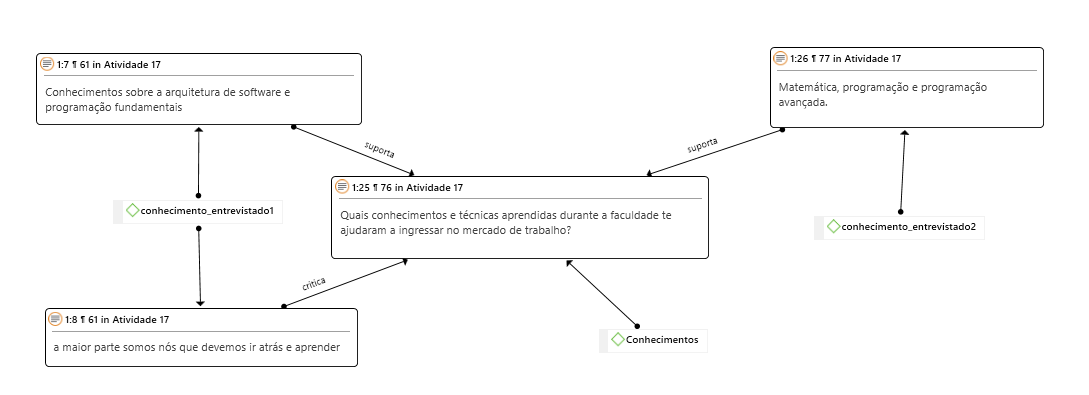
\includegraphics[width=16cm]{discuss/Conhecimentos.PNG}
        \caption{Codificação Axial -- Questão 3.}
        \label{fig:ca_q3}
    \end{figure}
    \FloatBarrier
    
    
    
    $\\$
    Proposições:
    \begin{itemize}
        \item P1. As empresas selecionam novos profissionais de T.I. com base em suas formações\cite{ref_3}\cite{ref_5}.
        \item P2. As empresas não levam muito em conta a formação dos profissionais\cite{ref_5}\cite{ref_4}\cite{ref_1}.
        \item P3. As empresas valorizam mais as atuações do profissional no mercado\cite{ref_3}\cite{ref_4}\cite{ref_2}.
        \item P4. As empresas selecionam o profissional com base na experiência em uma linguagem de programação\cite{ref_3}\cite{ref_4}.
    \end{itemize}

\fi